\section{Nearest neighbours}
\subsection{Classical nearest neighbours}
Figure~\ref{fig:knn} shows the results of the $k$-NN algorithm in function of the number of training data-points for a different number of neighbours. We can see that the performance is very similar to radial based function support vector machines.

A first observation is that at the contrary to SVMs models, the performance always keep increasing with added number of training points. This makes sense as support vector machines have a limited complexity due to their limited number of coefficients to be trained in their primal form. This is not totally true for SMVs using kernel functions and being evaluated in the dual, but their complexity is based on the number of support vectors which are consisting of only data-points close to the decision boundary. Adding more training points only improves the performance when those are close to the decision boundary if we neglect the smoothening of the boundary --- which in our case appears to be not very important. In $k$-NN algorithm, all data-points participate to the decision boundary. Augmenting the density of data-points allow the decision boundary to be influenced by any new data-point. The need for intricate boundaries --- or high complexity --- is also an explanation of the good performance of $k$-NN.

To understand the high variability of Matthew's correlation coefficient, we must have a more detailed look at the individual results (table~\ref{tab:knn-1} and \ref{tab:knn-2}). Matthew's correlation coefficient is computed on the binary correlation matrices for each class. For the total one, the mean is taken. As already mentioned before, the big advantage of this coefficient is that it takes into account the prior probabilities of both binary classes. This has a huge influence on the U2R class --- and in a lesser manner the R2L class --- that has very few instances. The accuracy is thus very good as very few points as classified in this category as should be for the very big majority, but the classifier is not very successful for the ones that should. As discussed before, not much can be done except from augmenting the instances of these classes.

The $k$-NN does as good as the best radial based function support vector machine for $n=10,000$ instances and surpasses all the previously tested algorithms for more training points, where this is very clear for $n=100,000$.

\begin{figure}[ht!]
        \begin{subfigure}[b]{.97\textwidth}  
            \centering 
            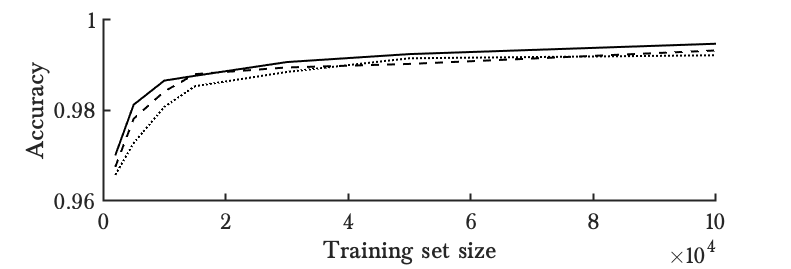
\includegraphics[width=.98\textwidth]{parts/chap-4/img-knn/knn-acc.png}
            \caption{Accuracy in function of the number of training points for a different number of neighbours.}
        \end{subfigure}
        \vfill
        \begin{subfigure}[b]{.97\textwidth}  
            \centering 
            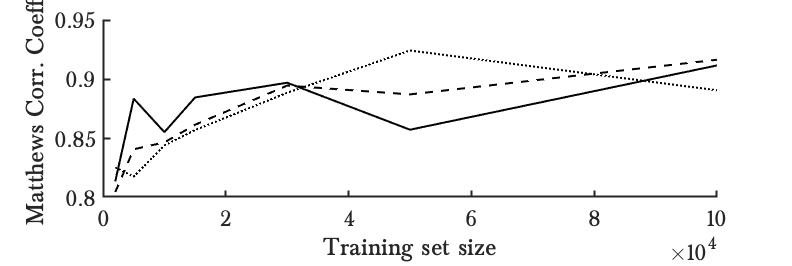
\includegraphics[width=.98\textwidth]{parts/chap-4/img-knn/knn-mcc.png}
            \caption{Matthew's correlation coefficient in function of the number of training points for a different number of neighbours.} 
        \end{subfigure}
        \vfill
        \begin{subfigure}[b]{.97\textwidth}  
            \centering 
            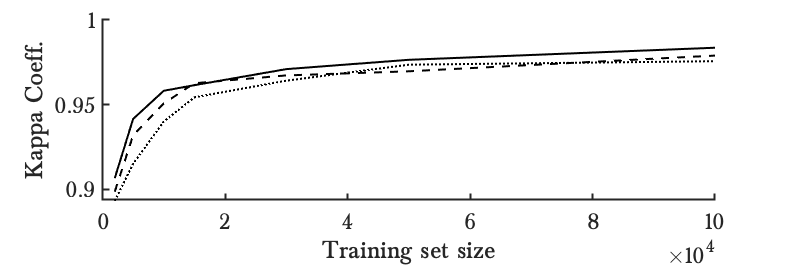
\includegraphics[width=.98\textwidth]{parts/chap-4/img-knn/knn-kappa.png}
            \caption{Cohen's kappa coefficient in function of the number of training points for a different number of neighbours.} 
        \end{subfigure}
        \vfill
        \caption{Performance of the $k$-NN algorithm in function of the number of training data-points for a different number of neighbours. The plain line is for $k=1$, the dashed is $k=2$ and the dotted is $k=3$.}
        \label{fig:knn}
\end{figure}

\begin{table}[ht!]
    \centering
    \begin{tabularx}{\textwidth}{lcccccccc}
    \hlineI
    Model &&& Normal & Probe & Dos & R2L & U2R & Total \\ \hlineI
    \multicolumn{9}{l}{$k=1$ with $n=10,000$}\\
    Accuracy [\%] &&& 98.17 & 99.45 & 98.80 & 98.03 & 43.33 & 98.66\\ 
    MCC [\%] &&& 97.49 & 99.19 & 98.63 & 92.76 & 39.68 & 85.55\\ 
    Kappa [\%] &&& 23.48 & 41.80 & 42.04 & 94.07 & 99.74 & 95.81\\    \hline
    Obs. Normal  &&& 2945 & 11 & 15 & 25 & 4 & \\ 
    Obs. Probe  &&& 10 & 2246 & 2 & 1 & 0 & \\ 
    Obs. DoS  &&& 23 & 3 & 2231 & 1 & 1 & \\ 
    Obs. R2L  &&& 2 & 0 & 0 & 214 & 2 & \\ 
    Obs. U2R  &&& 3 & 0 & 0 & 2 & 4 & \\  \hlineI
    
    \multicolumn{9}{l}{$k=2$ with $n=10,000$}\\
    Accuracy [\%] &&& 98.26 & 99.37 & 98.26 & 95.93 & 30 & 98.42\\ 
    MCC [\%]  &&& 97.08 & 98.86 & 98.44 & 90.31 & 38.74 & 84.69\\ 
    Kappa [\%] &&& 23.24 & 41.49 & 42.03 & 94.82 & 99.75 & 95.07\\  \hline
    Obs. Normal  &&& 2948 & 17 & 9 & 24 & 2 & \\ 
    Obs. Probe && & 12 & 2252 & 1 & 1 & 0 & \\ 
    Obs. DoS && & 34 & 5 & 2227 & 1 & 0 & \\ 
    Obs. R2L && & 6 & 0 & 0 & 181 & 1 & \\ 
    Obs. U2R && & 3 & 0 & 0 & 5 & 4 & \\ \hlineI
    
    \multicolumn{9}{l}{$k=3$ with $n=10,000$}\\
    Accuracy [\%] &&& 97.05 & 98.90 & 98.80 & 97.81 & 55.00 & 98.08\\ 
    MCC [\%] &&& 96.36 & 98.63 & 98.31 & 89.11 & 39.73 & 84.43\\ 
    Kappa [\%] &&& 24.10 & 41.88 & 41.87 & 94.06 & 99.69 & 94.00\\    \hline 
    Obs. Normal && & 2912 & 15 & 22 & 43 & 10 & \\ 
    Obs. Probe && & 18 & 2236 & 5 & 1 & 0 & \\ 
    Obs. DoS && & 22 & 4 & 2234 & 1 & 0 & \\ 
    Obs. R2L && & 3 & 0 & 0 & 205 & 2 & \\ 
    Obs. U2R && & 3 & 0 & 0 & 1 & 4 & \\  \hlineI
    \end{tabularx}
    \caption{Detailed results of the $k$-NN classification algorithm for two different values of the number of neighbours $k$ and for a big and a small training data-set. The accuracy, true positive rate (TP), true negative rate (TN), false positive rate (FP) and false negative rate (FN) are given for each target class.}
    \label{tab:knn-1}
\end{table}

\begin{table}[ht!]
    \centering
    \begin{tabularx}{\textwidth}{lcccccccc}
    \hlineI
    Model &&& Normal & Probe & Dos & R2L & U2R & Total \\ \hlineI
    \multicolumn{9}{l}{$k=1$ with $n=100,000$}\\
    Accuracy [\%] &&& 99.56 & 99.82 & 99.63 & 93.81 & 58.33 & 99.48\\ 
    MCC [\%] &&& 99.00 & 99.73 & 99.57 & 95.39 & 62.16 & 91.17\\ 
    Kappa [\%] &&& 22.61 & 41.51 & 41.58 & 94.88 & 99.85 & 98.36\\  \hline
    Obs. Normal  &&& 2987 & 4 & 4 & 5 & 1 & \\ 
    Obs. Probe  &&& 2 & 2260 & 2 & 0 & 0 & \\ 
    Obs. DoS  &&& 8 & 0 & 2256 & 0 & 0 & \\ 
    Obs. R2L  &&& 12 & 0 & 0 & 190 & 1 & \\ 
    Obs. U2R  &&& 2 & 0 & 0 & 1 & 4 & \\   \hlineI
    
    \multicolumn{9}{l}{$k=2$ with $n=100,000$}\\
    Accuracy [\%] &&& 99.19 & 99.92 & 99.57 & 94.32 & 48.89 & 99.33\\ 
    MCC [\%]  &&& 98.64 & 99.72 & 99.35 & 95.07 & 65.47 & 91.65\\ 
    Kappa [\%] &&& 22.86 & 41.52 & 41.64 & 94.73 & 99.82 & 97.90\\   \hline
    Obs. Normal  &&& 2976 & 7 & 11 & 7 & 0 & \\ 
    Obs. Probe && & 2 & 2260 & 0 & 0 & 0 & \\ 
    Obs. DoS && & 9 & 1 & 2252 & 0 & 0 & \\ 
    Obs. R2L && & 12 & 0 & 0 & 194 & 0 & \\ 
    Obs. U2R && & 4 & 0 & 0 & 1 & 4 & \\ \hlineI
    
    \multicolumn{9}{l}{$k=3$ with $n=100,000$}\\
    Accuracy [\%] &&& 99.32 & 99.77 & 99.66 & 89.85 & 40.83 & 99.22\\ 
    MCC [\%] &&& 98.48 & 99.65 & 99.37 & 93.37 & 54.52 & 89.08\\ 
    Kappa [\%] &&& 22.71 & 41.52 & 41.52 & 95.11 & 99.77 & 97.56\\   \hline 
    Obs. Normal && & 2980 & 5 & 10 & 4 & 1 & \\ 
    Obs. Probe && & 4 & 2259 & 2 & 0 & 0 & \\ 
    Obs. DoS && & 8 & 0 & 2256 & 0 & 0 & \\ 
    Obs. R2L && & 19 & 1 & 0 & 177 & 0 & \\ 
    Obs. U2R && & 6 & 0 & 1 & 1 & 5 & \\  \hlineI
    \end{tabularx}
    \caption{Detailed results of the $k$-NN classification algorithm for two different values of the number of neighbours $k$ and for a big and a small training data-set. The accuracy, true positive rate (TP), true negative rate (TN), false positive rate (FP) and false negative rate (FN) are given for each target class.}
    \label{tab:knn-2}
\end{table}


\subsection{Training set reduction}
The training is linearly dependent on the number of instances in the training set --- the ones that are compared to to search for the nearest neighbours. To reduce the evaluation time, we must find a way to reduce this number and the find only the relevant data-points.

\subsubsection{$k$-means clustering}
\begin{wrapfigure}[13]{r}{0.45\textwidth}
\begin{center}
    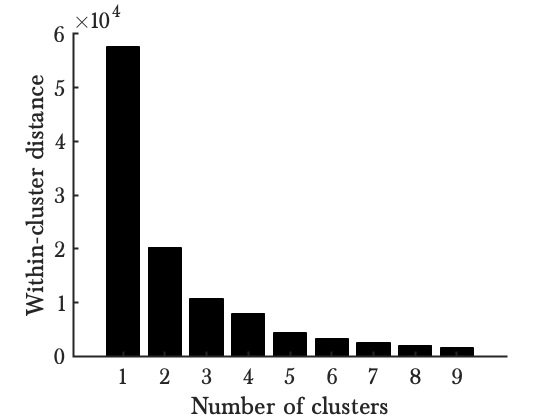
\includegraphics[width=.45\textwidth]{parts/chap-4/img-knn/kmeans.png}
    \caption{Within cluster sum of distances in function of the number of clusters chosen.}
    \label{fig:kmeans}
\end{center}
\end{wrapfigure}
To select the number of clusters, the elbow rule suggests to take 5 clusters, which is by the way the same results obtained by \cite{Soheily-Khah2018IntrusionDataset}, but with a different data-set (figure~\ref{fig:kmeans}). We can then only keep the normal instances near the decision boundary, i.e. the cluster with the closest mean to the other classes. This gives very disappointing results indipendently of the number of nearest neighbours $k$ chosen. Table~\ref{tab:knn-kmeans} also shows the results where the sole most-distant cluster is discarded. However, the results are still very disappointing although logically better than keeping the sole best cluster, we can see that a lot of normal data-points are abusively considered as various attacks. The model lacks information about the variety of normal attacks, variety that we just supressed.
This suggests that they are no specific regions where the data-points are not relevant. In other words, the decision boundary goes through all clusters, all regions of the hyper-space where points are present. This once again confirms the complexity of the decision boundary and the problem in general. We could try to augment the number of clusters to discard smaller groups and do this iteratively always discard the worse one, but after all, the direction this is going to is select the points individually and based on group methods. This problem is better tackled with condensed nearest neighbours.

\begin{table}[ht!]
    \centering
    \begin{tabularx}{\textwidth}{lcccccccc}
    \hlineI
    Model &&& Normal & Probe & Dos & R2L & U2R & Total \\ \hlineI
    \multicolumn{9}{l}{$k=1$ with $n=100,000$}\\
    Accuracy [\%] &&& 95.19 & 99.29 & 98.78 & 96.92 & 76 & 97.45\\ 
    MCC [\%] &&& 94.88 & 97.05 & 98.29 & 89.79 & 74.85 & 90.97\\ 
    Kappa [\%] &&& 25.09 & 41.02 & 41.67 & 94.85 & 99.60 & 92.02\\   \hline
    Obs. Normal  &&& 2856 & 12 & 25 & 5 & 3 & \\ 
    Obs. Probe  &&& 84 & 2251 & 2 & 0 & 0 & \\ 
    Obs. DoS  &&& 23 & 4 & 2239 & 0 & 0 & \\ 
    Obs. R2L  &&& 34 & 1 & 0 & 179 & 0 & \\ 
    Obs. U2R  &&& 4 & 0 & 0 & 0 & 11 & \\   \hlineI
    
    \multicolumn{9}{l}{$k=2$ with $n=100,000$}\\
    Accuracy [\%] &&& 95.03 & 99.26 & 98.28 & 97.82 & 55.00 & 97.27\\ 
    MCC [\%]  &&& 94.59 & 97.16 & 97.86 & 89.90 & 33.75 & 82.65\\ 
    Kappa [\%] &&& 25.26 & 41.32 & 42.08 & 93.91 & 99.82 & 91.48\\    \hline
    Obs. Normal  &&& 2851 & 13 & 34 & 4 & 1 & \\ 
    Obs. Probe && & 73 & 2243 & 5 & 0 & 0 & \\ 
    Obs. DoS && & 27 & 3 & 2221 & 0 & 0 & \\  
    Obs. R2L && & 43 & 1 & 0 & 211 & 1 & \\ 
    Obs. U2R && & 6 & 0 & 0 & 1 & 2 & \\  \hlineI
    
    \multicolumn{9}{l}{$k=3$ with $n=100,000$}\\
    Accuracy [\%] &&& 86.61 & 98.75 & 98.54 & 98.14 & 72.22 & 93.94\\
    MCC [\%] &&& 87.98 & 93.01 & 96.85 & 82.97 & 61.41 & 84.44\\ 
    Kappa [\%] &&& 29.48 & 40.32 & 41.77 & 93.22 & 99.72 & 81.06\\    \hline 
    Obs. Normal && & 2598 & 22 & 25 & 2 & 2 & \\ 
    Obs. Probe && & 246 & 2229 & 4 & 0 & 0 & \\ 
    Obs. DoS && & 65 & 5 & 2224 & 0 & 0 & \\ 
    Obs. R2L && & 87 & 1 & 4 & 216 & 1 & \\
    Obs. U2R && & 4 & 0 & 0 & 2 & 7 & \\  \hlineI
    \end{tabularx}
    \caption{Detailed results of the $k$-NN classification algorithm for two different values of the number of neighbours $k$ and for a big and a small training data-set. The accuracy, true positive rate (TP), true negative rate (TN), false positive rate (FP) and false negative rate (FN) are given for each target class.}
    \label{tab:knn-kmeans}
\end{table}

\subsubsection{Condensed nearest neighbours}
The clustering-based methods give good results for huge data-sets and \cite{Soheily-Khah2018IntrusionDataset} has successfully applied it to \emph{random forest classifiers}. In our case, we have a lesser number of data-points and we do not try to discard the majority of them, but intelligently select the relevant ones to reduce our number of instances in the training data-set. The condensed nearest neighbours is an instance-wise selection method and not based on larger groups as are clustering methods. However, the better results of the $k=1$ does not allow us to discard the outliers. Table~\ref{} shows the results of the condensed nearest neighbours.

\begin{figure}[ht!]
        \begin{subfigure}[b]{.97\textwidth}  
            \centering 
            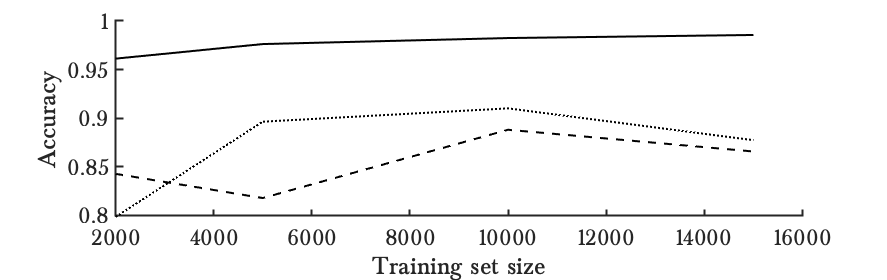
\includegraphics[width=.98\textwidth]{parts/chap-4/img-knn/cnn/acc.png}
            \caption{Accuracy with condensed nearest neighbours.}
        \end{subfigure}
        \vfill
        \begin{subfigure}[b]{.97\textwidth}  
            \centering 
            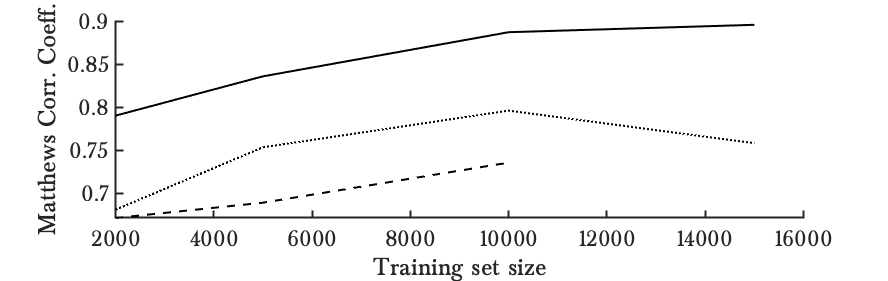
\includegraphics[width=.98\textwidth]{parts/chap-4/img-knn/cnn/mcc.png}
            \caption{Matthew's correlation coefficient with condensed nearest neighbours.} 
        \end{subfigure}
        \vfill
        \begin{subfigure}[b]{.97\textwidth}  
            \centering 
            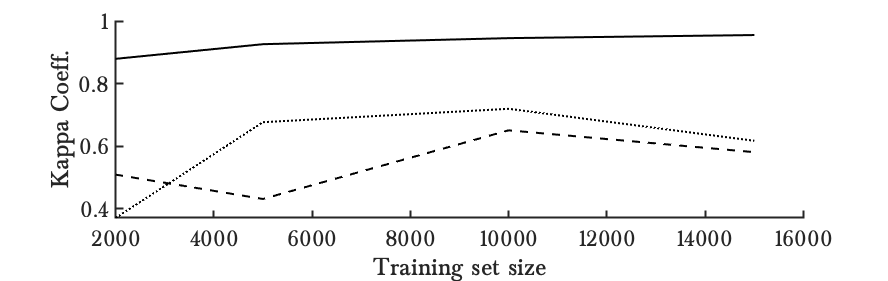
\includegraphics[width=.98\textwidth]{parts/chap-4/img-knn/cnn/kappa.png}
            \caption{Cohen's kappa coefficient with condensed neighbours.} 
        \end{subfigure}
        \vfill
        \begin{subfigure}[b]{.97\textwidth}  
            \centering 
            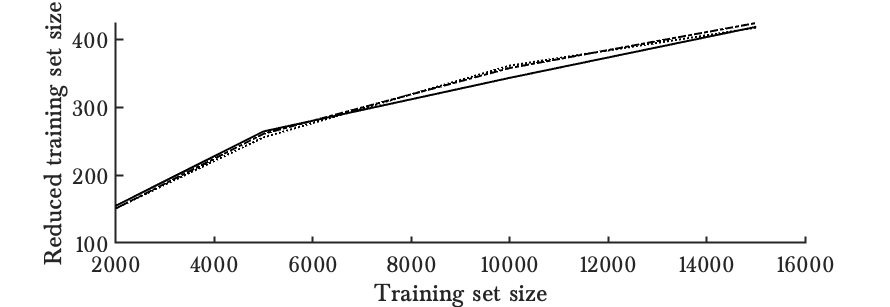
\includegraphics[width=.98\textwidth]{parts/chap-4/img-knn/cnn/red.png}
            \caption{Number of data-points after reduction.} 
        \end{subfigure}
        \caption{Performance of the $k$-NN algorithm in function of the number of training data-points for a different number of neighbours. The plain line is for $k=1$, the dashed is $k=2$ and the dotted is $k=3$.}
        \label{fig:knn-cnn}
\end{figure}

\begin{table}[ht!]
    \centering
    \begin{tabularx}{\textwidth}{lcccccccc}
    \hlineI
    Model &&& Normal & Probe & Dos & R2L & U2R & Total \\ \hlineI
    \multicolumn{9}{l}{$k=1$ with $n=10,000$}\\
    Accuracy [\%] &&& 97.63 & 99.11 & 98.26 & 98.16 & 80 & 98.25\\ 
    MCC [\%] &&& 96.73 & 99.02 & 98.02 & 90.27 & 59.45 & 88.70\\ 
    Kappa [\%] &&& 23.74 & 41.94 & 42.19 & 93.92 & 99.70 & 94.52\\    \hline
    Obs. Normal  &&& 2929 & 14 & 31 & 3 & 1 & \\ 
    Obs. Probe  &&& 9 & 2238 & 1 & 1 & 0 & \\ 
    Obs. DoS  &&& 20 & 4 & 2219 & 0 & 0 & \\ 
    Obs. R2L  &&& 36 & 1 & 4 & 213 & 1 & \\ 
    Obs. U2R  &&& 6 & 0 & 3 & 0 & 6 & \\    \hlineI
    
    \multicolumn{9}{l}{$k=2$ with $n=10,000$}\\
    Accuracy [\%] &&& 93.67 & 94.48 & 78.75 & 68.56 & 36.67 & 88.81\\ 
    MCC [\%]  &&& 85.64 & 84.77 & 82.47 & 78.84 & 36.00 & 73.54\\ 
    Kappa [\%] &&& 24.58 & 40.61 & 48.94 & 95.17 & 99.86 & 65.03\\     \hline
    Obs. Normal  &&& 2810 & 44 & 238 & 66 & 2 & \\ 
    Obs. Probe && & 172 & 2135 & 241 & 0 & 0 & \\ 
    Obs. DoS && & 6 & 81 & 1780 & 0 & 0 & \\ 
    Obs. R2L && & 10 & 0 & 1 & 147 & 2 & \\ 
    Obs. U2R && & 2 & 0 & 0 & 1 & 2 & \\   \hlineI
    
    \multicolumn{9}{l}{$k=3$ with $n=10,000$}\\
    Accuracy [\%] &&& 94.37 & 90.02 & 88.40 & 86.43 & 36.47 & 91.01\\ 
    MCC [\%] &&& 90.39 & 85.97 & 85.30 & 85.11 & 51.17 & 79.59\\ 
    Kappa [\%] &&& 25.04 & 43.77 & 44.66 & 94.26 & 99.67 & 71.91\\    \hline 
    Obs. Normal &&& 2831 & 41 & 106 & 29 & 10 & \\ 
    Obs. Probe && & 101 & 2029 & 155 & 0 & 0 & \\ 
    Obs. DoS &&& 35 & 182 & 1993 & 0 & 0 & \\ 
    Obs. R2L &&& 32 & 2 & 1 & 191 & 0 & \\ 
    Obs. U2R &&& 1 & 0 & 0 & 1 & 6 & \\   \hlineI
    \end{tabularx}
    \caption{Detailed results of the $k$-NN classification algorithm for two different values of the number of neighbours $k$ and for a big and a small training data-set. The accuracy, true positive rate (TP), true negative rate (TN), false positive rate (FP) and false negative rate (FN) are given for each target class.}
    \label{tab:knn-cnn}
\end{table}

\subsection{Feature size reduction}

\subsubsection{Principal components analysis}



\subsubsection{$\chi^2$ feature selection}